\documentclass{article}
\usepackage{cmap}
\usepackage[utf8]{inputenc}
\usepackage[english,ukrainian]{babel}
\usepackage{graphicx}
\usepackage{geometry}
\usepackage{listings}
\usepackage{amsmath}
\usepackage{float}
\geometry{
	a4paper,
	left=20mm,
	right=20mm,
	top=20mm,
	bottom=20mm
}
\lstset{
	language=c++,
	tabsize=4,
	keepspaces,
	showstringspaces=false,
	breaklines,
}
\graphicspath{ {./pictures} }
\setlength{\parindent}{4em}

\newcommand\subject{Операційні системи}
\newcommand\lecturer{старший викладач кафедри ПЗ\\Грицай О.Д.}
\newcommand\teacher{старший викладач кафедри ПЗ\\Грицай О.Д.}
\newcommand\mygroup{ПЗ-22}
\newcommand\lab{8}
\newcommand\theme{Управління файловою системою}
\newcommand\purpose{Ознайомитися з файловими системами операційних систем Windows та
	LINUX}

\begin{document}
\begin{normalsize}
	\begin{titlepage}
		\thispagestyle{empty}
		\begin{center}
			\textbf{МІНІСТЕРСТВО ОСВІТИ І НАУКИ УКРАЇНИ\\
				НАЦІОНАЛЬНИЙ УНІВЕРСИТЕТ "ЛЬВІВСЬКА ПОЛІТЕХНІКА"}
		\end{center}
		\begin{flushright}
			Інститут \textbf{КНІТ}\\
			Кафедра \textbf{ПЗ}
		\end{flushright}
		\vspace{200pt}
		\begin{center}
			\textbf{ЗВІТ}\\
			\vspace{10pt}
			До лабораторної роботи № \lab\\
			\textbf{На тему}: “\textit{\theme}”\\
			\textbf{З дисципліни}: “\subject”
		\end{center}
		\vspace{112pt}
		\begin{flushright}
			
			\textbf{Лектор}:\\
			\lecturer\\
			\vspace{28pt}
			\textbf{Виконав}:\\
			
			студент групи \mygroup\\
			Коваленко Д.М.\\
			\vspace{28pt}
			\textbf{Прийняла}:\\
			
			\teacher\\
			
			\vspace{28pt}
			«\rule{1cm}{0.15mm}» \rule{1.5cm}{0.15mm} 2022 р.\\
			$\sum$ = \rule{1cm}{0.15mm}……………\\
			
		\end{flushright}
		\vspace{\fill}
		\begin{center}
			\textbf{Львів — 2022}
		\end{center}
	\end{titlepage}
		
	\begin{description}
		\item[Тема.] \theme.
		\item[Мета.] \purpose.
	\end{description}

	\section*{Лабораторне завдання}
	
	\begin{figure}[H]
		\centering
		
\includegraphics[scale=0.5]{v}
	\end{figure}
	\begin{center}
		2. Вивести посортовані по зростанню методом «бульбашки» рядки
		матриці матриці N*N (N>1000 задається користувачем, матриця
		визначається випадково).
	\end{center}

	\section*{Хід роботи}	
	\section*{WINDOWS}
	\textbf{main.cpp}
	\begin{lstlisting}
#include <iostream>
#include <fstream>
#include <string>
#include <vector>
#include <Windows.h>

#define N 100

using namespace std;

void task(HANDLE handle);
vector<string> split(string s, string delimiter);
void bubble_sort(int* array);

int main() {
	string filename;
	HANDLE handle;
	cout << "Enter file name: ";
	cin >> filename;
	filename = "C:\\Users\\Dmytro\\source\\repos\\os8\\" + filename;
	handle = CreateFileA((LPCSTR)filename.c_str(), GENERIC_WRITE, NULL, NULL, CREATE_ALWAYS, FILE_ATTRIBUTE_NORMAL, NULL);
	
	if (handle == INVALID_HANDLE_VALUE)
	return -1;
	
	task(handle);
	
	CloseHandle(handle);
	
	bool exit = true;
	while (exit) {
		int desired_attrs;
		DWORD attrs = GetFileAttributesA((LPCSTR)filename.c_str());
		if (attrs == NULL) {
			cout << "null" << endl;
		}
		cout << "Enter file attributes to set: \n[1]-reset,\n[2]-readonly,\n[3]-hidden\n";
		cin >> desired_attrs;
		switch (desired_attrs) {
			case 1:
			attrs = attrs & ~FILE_ATTRIBUTE_READONLY & ~FILE_ATTRIBUTE_HIDDEN;
			break;
			case 2:
			attrs = attrs | FILE_ATTRIBUTE_READONLY;
			break;
			case 3:
			attrs = attrs | FILE_ATTRIBUTE_HIDDEN;
			break;
		}
		SetFileAttributesA((LPCSTR)filename.c_str(), attrs);
	}
}

void task(HANDLE handle) 
{
	int** array = new int* [N];
	for (int i = 0; i < N; i++) array[i] = new int[N];
	
	std::srand(static_cast<unsigned int>(std::time(nullptr)));
	for (int i = 0; i < N; i++)
	{
		for (int j = 0; j < N; j++)
		{
			array[i][j] = rand();
		}
	}
	
	for (int i = 0; i < N; i++)
	{
		bubble_sort(array[i]);
	}
	
	string text;
	for (int i = 0; i < N; i++)
	{
		for (int j = 0; j < N; j++)
		{
			if (j == N - 1)
			text += to_string(array[i][j]);
			else
			text += to_string(array[i][j]);
			text += ",";
		}
		text += "\n";
	}
	WriteFile(handle, text.c_str(), text.size(), NULL, NULL);
}

void bubble_sort(int* array)
{
	for (int i = 0; i < N; i++)
	{
		for (int j = 0; j < N - i - 1; j++)
		{
			if (array[j] > array[j + 1])
			{
				swap(array[j], array[j + 1]);
			}
		}
	}
}

vector<string> split(string s, string delimiter) {
	size_t pos_start = 0, pos_end, delim_len = delimiter.length();
	string token;
	vector<string> res;
	
	while ((pos_end = s.find(delimiter, pos_start)) != string::npos) {
		token = s.substr(pos_start, pos_end - pos_start);
		pos_start = pos_end + delim_len;
		res.push_back(token);
	}
	
	res.push_back(s.substr(pos_start));
	return res;
}

	\end{lstlisting}
	
	\begin{figure}[H]
		\centering
		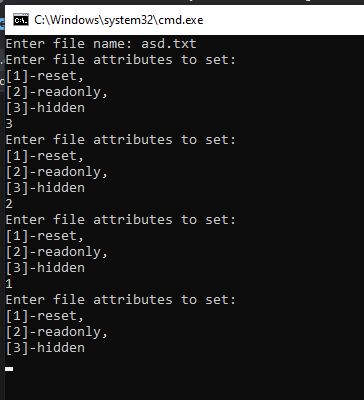
\includegraphics[scale=0.9]{1}
		\caption{Виконання програми windows}
	\end{figure}

\section*{LINUX}
\textbf{main.cpp}
\begin{lstlisting}
#include <iostream>
#include <fstream>
#include <string>
#include <vector>
#include <sys/stat.h>
#include <unistd.h>
#include <fcntl.h>

#define N 100

using namespace std;

void task(int file);
vector<string> split(string s, string delimiter);
void bubble_sort(int* array);

int main() {
	string filename;
	cout << "Enter file name: ";
	cin >> filename;
	int mode = S_IRUSR | S_IRGRP | S_IROTH;
	int file = open(filename.c_str(), O_RDWR | O_CREAT, mode);
	
	if (file == -1) {
		cout << "open() error" << endl;
	}
	
	task(file);
	
	close(file);
	
	bool exit = true;
	while (exit) {
		int desired_attrs;
		cout << "Enter file attributes to set: ";
		cin >> desired_attrs;
		switch (desired_attrs) {
			case 1:
			mode = mode | S_IXOTH;
			break;
			case 2:
			mode = mode | S_IWOTH;
			break;
			case 4:
			mode = mode | S_IROTH;
			break;
			case 7:
			mode = mode | S_IRWXO;
			break;
			case 10:
			mode = mode | S_IXGRP;
			break;
			case 20:
			mode = mode | S_IWGRP;
			break;
			case 40:
			mode = mode | S_IRGRP;
			break;
			case 70:
			mode = mode | S_IRWXG;
			break;
			case 100:
			mode = mode | S_IXUSR;
			break;
			case 200:
			mode = mode | S_IWUSR;
			break;
			case 400:
			mode = mode | S_IRUSR;
			break;
			case 700:
			mode = mode | S_IRWXU;
			break;
		}
		chmod(filename.c_str(), mode);
	}
}

void task(int file) 
{
	int** array = new int* [N];
	for (int i = 0; i < N; i++) array[i] = new int[N];
	
	srand(static_cast<unsigned int>(time(nullptr)));
	for (int i = 0; i < N; i++)
	{
		for (int j = 0; j < N; j++)
		{
			array[i][j] = rand();
		}
	}
	
	for (int i = 0; i < N; i++)
	{
		bubble_sort(array[i]);
	}
	
	string text;
	for (int i = 0; i < N; i++)
	{
		for (int j = 0; j < N; j++)
		{
			if (j == N - 1)
			text += to_string(array[i][j]);
			else
			text += to_string(array[i][j]);
			text += ",";
		}
		text += "\n";
	}
	write(file, text.c_str(), text.size());
}

void bubble_sort(int* array)
{
	for (int i = 0; i < N; i++)
	{
		for (int j = 0; j < N - i - 1; j++)
		{
			if (array[j] > array[j + 1])
			{
				swap(array[j], array[j + 1]);
			}
		}
	}
}

vector<string> split(string s, string delimiter) {
	size_t pos_start = 0, pos_end, delim_len = delimiter.length();
	string token;
	vector<string> res;
	
	while ((pos_end = s.find(delimiter, pos_start)) != string::npos) {
		token = s.substr(pos_start, pos_end - pos_start);
		pos_start = pos_end + delim_len;
		res.push_back(token);
	}
	
	res.push_back(s.substr(pos_start));
	return res;
}
\end{lstlisting}

\begin{figure}[H]
	\centering
	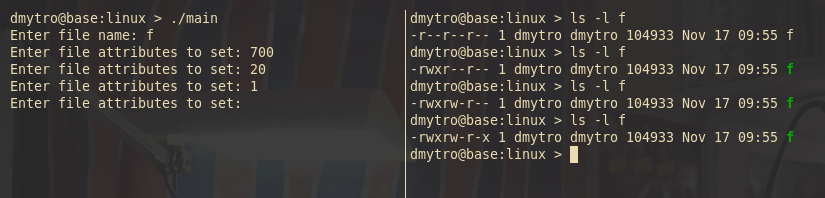
\includegraphics[scale=0.6]{2}
	\caption{Виконання програми Linux}
\end{figure}
	
	\section*{Висновок}
	Під час виконання лабораторної роботи я ознайомився з файловими системами операційних систем Windows та LINUX.
	
	 
\end{normalsize}
\end{document}
